\documentclass[12pt]{article}

\usepackage{sbc-template}
\usepackage[T1]{fontenc}
\usepackage[utf8]{inputenc}
\usepackage[brazilian]{babel}
\usepackage{graphicx,url}
\usepackage{float}
\usepackage{multirow}
\usepackage[none]{hyphenat}
\usepackage{tikz}
\usetikzlibrary{positioning,arrows.meta}

\sloppy
\hyphenpenalty=10000
\exhyphenpenalty=10000
\emergencystretch=3em
\setlength{\textfloatsep}{6pt}
\setlength{\floatsep}{6pt}
\setlength{\intextsep}{6pt}
\setlength{\abovecaptionskip}{4pt}
\setlength{\belowcaptionskip}{0pt}
\setlength{\parskip}{2pt}

\title{Um \textit{Pipeline} de Vis\~ao Computacional para Caracteriza\c{c}\~ao de Achados Intrarrenais em Ultrassonografia}

\author{
  Jefferson S. dos Anjos\inst{1}, Amaro A. de Lima\inst{1},
  Gabriel M. Ara\'ujo\inst{1},\\ Jorge Luiz de C. Henriques Junior\inst{2},
  Norderval C. Ara\'ujo\inst{2}, Jos\'e Herm\'ogenes R. Suassuna\inst{2},\\ Felipe da R. Henriques\inst{1}
}

\address{
  CEFET/RJ -- Rio de Janeiro -- RJ -- Brasil\\
  $^{2}$ HUPE -- UERJ -- Rio de Janeiro -- RJ -- Brasil\\
\vspace{-0.7cm}
\email{jefferson.anjos.1@aluno.cefet-rj.br,}\\
\vspace{-0.7cm}  \email{\{amaro.lima,gabriel.araujo,felipe.henriques\}@cefet-rj.br},\\
\vspace{-0.7cm}  \email{\{jorge.henriques,norderval.norderval\}@uerj.br}
}

\begin{document}

\maketitle

\begin{abstract}
Renal ultrasound interpretation depends on subjective visual inspection and anatomical delimitation of the kidney. This paper proposes a computer vision \textit{pipeline} that first segments the kidney and then extracts exploratory intrarenal echogenicity and texture markers. An exploratory annotated set was used to train an initial model, which generated pseudo masks accepted only above a 90\% operational confidence threshold. After data expansion, a second DeepLabV3 ResNet50 model was trained on the consolidated set and achieved Dice of 0.9235, IoU of 0.8741 and precision of 0.9301 on a fixed test set. Fibrosis, commonly assessed histologically as interstitial fibrosis and tubular atrophy (IFTA), is not a validated outcome in the current dataset.
\end{abstract}

\begin{resumo}
A interpreta\c{c}\~ao de ultrassonografias renais depende de inspe\c{c}\~ao visual subjetiva e da delimita\c{c}\~ao anat\^omica do rim. Este artigo prop\~oe um \textit{pipeline} de vis\~ao computacional que primeiro segmenta o rim e depois extrai marcadores explorat\'orios de ecogenicidade e textura intrarrenal. Uma base explorat\'oria anotada foi usada para treinar um modelo inicial, que gerou pseudom\'ascaras aceitas apenas acima de 90\% de confian\c{c}a operacional. Ap\'os a expans\~ao dos dados, um segundo DeepLabV3 ResNet50 foi treinado no conjunto consolidado e atingiu Dice de 0,9235, IoU de 0,8741 e precis\~ao de 0,9301 no teste fixo. Fibrose, usualmente avaliada histologicamente como fibrose intersticial e atrofia tubular (IFTA), n\~ao constitui um desfecho validado na base atual.
\end{resumo}

\section{Introdu\c{c}\~ao}

A ultrassonografia renal \'e acess\'ivel, n\~ao invasiva e amplamente usada na avalia\c{c}\~ao de altera\c{c}\~oes estruturais do rim. Na pr\'atica cl\'inica, ecogenicidade cortical, dimens\~oes renais e diferencia\c{c}\~ao cortico-medular podem contribuir para avaliar altera\c{c}\~oes parenquimatosas, embora n\~ao determinem isoladamente fibrose.

Em estudos pareados com bi\'opsia, o desfecho de fibrose \'e frequentemente operacionalizado como \textit{interstitial fibrosis and tubular atrophy} (IFTA). Moghazi et al.~\cite{Moghazi2005} mostraram que a ecogenicidade cortical correlaciona-se com achados histopatol\'ogicos, mas possui especificidade limitada quando usada isoladamente. Athavale et al.~\cite{Athavale2021} demonstraram a viabilidade de predizer classes de IFTA a partir de ultrassonografia, utilizando r\'otulos histol\'ogicos como padr\~ao de refer\^encia.

A ecogenicidade cortical, especialmente quando comparada ao fígado, também é
observada em pacientes com doença renal crônica. A razão entre a intensidade cortical
renal e a intensidade de um órgão de referência pode reduzir parte da subjetividade da
inspeção visual~\cite{Manley2001}.

Em paralelo, a literatura explora segmentação renal e extração de medidas
quantitativas de intensidade e textura para investigar padr\~oes associados a altera\c{c}\~oes
renais~\cite{Athavale2021}. Ainda assim, permanece a lacuna entre segmentar o rim e examinar, dentro dele, pontos hiperecog\^enicos candidatos a achados suspeitos.

Esse recorte \'e importante porque a ultrassonografia apresenta ru\'ido, sombras ac\'usticas, varia\c{c}\~oes de ganho e diferen\c{c}as de enquadramento. Sem uma m\'ascara renal confi\'avel, pontos muito claros podem ser confundidos com artefatos ou estruturas externas ao rim. Por isso, este trabalho parte da delimita\c{c}\~ao sem\^antica do rim e s\'o depois transforma achados hiperecog\^enicos em medidas computacionais.

Este artigo combina segmenta\c{c}\~ao renal, expans\~ao supervisionada por pseudom\'ascaras e extra\c{c}\~ao de atributos intrarrenais. As contribui\c{c}\~oes s\~ao: consolida\c{c}\~ao de acervo expandido, gera\c{c}\~ao de pseudom\'ascaras com limiar de 90\%, treinamento de um segundo segmentador e avalia\c{c}\~ao explorat\'oria de marcadores ultrassonogr\'aficos intrarrenais.

\section{Contexto e Trabalhos Relacionados}

A segmenta\c{c}\~ao autom\'atica de rim em ultrassonografia \'e a primeira linha relacionada a este estudo. Arquiteturas como \mbox{U-Net}~\cite{Ronneberger2015}, DeepLabV3~\cite{Chen2018DeepLab} e SegFormer~\cite{Xie2021SegFormer} preservam bordas, capturam contexto multiescala e lidam com varia\c{c}\~oes de textura.

A segunda linha é a quantificação da ecogenicidade renal relativa, em que medidas
entre rim e fígado aproximam critérios usados por especialistas~\cite{Manley2001}.A terceira
é a extração de atributos quantitativos relacionados à textura e intensidade da imagem
para investigacao de alteracoes renais~\cite{Athavale2021}.

Estruturas intrarrenais candidatas s\~ao mantidas apenas como refer\^encias espaciais explorat\'orias; elas n\~ao s\~ao tratadas, neste estudo, como marcador direto de IFTA.

Em segmenta\c{c}\~ao, Dice e IoU medem a sobreposi\c{c}\~ao entre m\'ascara prevista e refer\^encia. Ambas variam de 0 a 1: valores pr\'oximos de 0 indicam baixa concord\^ancia, e valores pr\'oximos de 1 indicam maior proximidade entre predi\c{c}\~ao e anota\c{c}\~ao esperada.

\section{Metodologia}

A metodologia foi organizada para transformar uma imagem de ultrassonografia renal em uma regi\~ao anat\^omica delimitada e, em seguida, extrair marcadores explorat\'orios de intensidade e textura intrarrenal.

Para isso, o \textit{pipeline} primeiro prepara a entrada, segmenta o rim, restringe a an\'alise \`a m\'ascara renal, procura regi\~oes claras intrarrenais e, por fim, produz marcadores quantitativos. Uma eventual predi\c{c}\~ao de IFTA exige dados associados a bi\'opsia ou refer\^encia cl\'inica validada e fica fora do escopo demonstrado. A Figura~\ref{fig:tikz_pipeline} apresenta essa organiza\c{c}\~ao geral.

\begin{figure}[htb!]
\centering
\begin{tikzpicture}[
    node distance=0.45cm and 0.45cm,
    >=Latex,
    every node/.style={font=\footnotesize, align=center},
    block/.style={draw, rounded corners=2pt, minimum width=2.35cm, minimum height=0.72cm, fill=gray!8}
]
\node[block] (input) {Imagem de\\ultrassom};
\node[block, right=of input] (prep) {Preparo da\\entrada};
\node[block, right=of prep] (seg) {Segmenta\c{c}\~ao\\renal};
\node[block, right=of seg] (feat) {Regi\~oes claras\\intrarrenais};
\node[block, right=of feat] (clf) {Marcadores\\explorat\'orios};
\draw[->, thick] (input) -- (prep);
\draw[->, thick] (prep) -- (seg);
\draw[->, thick] (seg) -- (feat);
\draw[->, thick] (feat) -- (clf);
\end{tikzpicture}
\caption{\textit{Pipeline} metodol\'ogico: a segmenta\c{c}\~ao renal isola o rim para extra\c{c}\~ao explorat\'oria de marcadores intrarrenais.}
\label{fig:tikz_pipeline}
\end{figure}

Como indicado na Figura~\ref{fig:tikz_pipeline}, a primeira etapa recebe a imagem de ultrassonografia, aplica normalização e redimensionamento e prepara a entrada para o segmentador. A segunda etapa segmenta o rim e usa a máscara resultante como janela anatômica, reduzindo falsos candidatos fora do órgão.

Na terceira etapa, a imagem em tons de cinza é examinada apenas dentro dessa região, buscando concentra\c{c}\~oes locais de pixels de alta intensidade próximas a regiões internas candidatas às pir\^amides.Em seguida, são extraídos atributos de intensidade,
dispersão, percentis, proporção de pixels brilhantes e textura por matrizes de coocorrência de níveis de cinza~\cite{Haralick1973}.

Quando h\'a ROI manual do f\'igado, tamb\'em s\~ao calculadas raz\~oes entre rim e f\'igado. A etapa final usa um Random Forest~\cite{Breiman2001} apenas como prova de conceito de separa\c{c}\~ao de marcadores imag\'eticos; os r\'otulos dispon\'iveis n\~ao representam IFTA confirmada.

O desenvolvimento foi organizado em duas fases. Na primeira, a base explorat\'oria derivada do Open Kidney Ultrasound Data Set~\cite{Singla2023KidneyUS} reuniu 513 pares imagem e m\'ascara, distribu\'idos em 360 imagens de treino, 51 de valida\c{c}\~ao e 102 de teste. Esse conjunto treinou o modelo inicial, respons\'avel por aprender o contorno renal.

Na segunda fase, o acervo foi ampliado com imagens locais e externas. O maior acr\'escimo veio do MONAI Clinical Ultrasound Image Repository: como o reposit\'orio completo \'e amplo e heterog\^eneo, foram filtrados nos metadados apenas estudos renais ou retroperitoneais. Os DICOMs selecionados foram convertidos para PNG, com descarte de quadros RGB ou coloridos para evitar Doppler e imagens fora do padr\~ao B-mode. A curadoria gerou 4.487 PNGs; ap\'os deduplica\c{c}\~ao, 4.479 entraram no \texttt{dataset\_geral}.

Para explicitar essa constru\c{c}\~ao do acervo, a Tabela~\ref{tab:data_evolution} resume os blocos que alimentaram o conjunto consolidado usado no segundo treinamento.

\begin{table}[H]
\centering
\caption{Composi\c{c}\~ao do acervo consolidado para segmenta\c{c}\~ao renal.}
\label{tab:data_evolution}
\begin{tabular}{lcc}
\hline
\textbf{Origem} & \textbf{Imagens} & \textbf{Papel no acervo} \\
\hline
Open Kidney / \texttt{kidneyUS} & 513 & base inicial manual \\
Subconjuntos locais & 1.002 & complemento organizado \\
MONAI renal curado & 4.479 & expans\~ao externa \\
\textbf{Total} & \textbf{5.994} & \texttt{dataset\_geral} \\
\hline
\end{tabular}
\end{table}

Como mostrado na Tabela~\ref{tab:data_evolution}, o \texttt{dataset\_geral} combina a base Open Kidney/\texttt{kidneyUS}, subconjuntos locais e o subconjunto MONAI curado. As imagens sem m\'ascara manual foram pseudorrotuladas~\cite{Lee2013PseudoLabel}, e as novas m\'ascaras s\'o foram aceitas quando a predi\c{c}\~ao atingiu confian\c{c}a operacional de pelo menos 90\% e passou por filtros de \'area, componentes conectados e pixels de primeiro plano.

Na vers\~ao usada nos experimentos relatados, 3.962 imagens tinham m\'ascaras aceitas: 1.001 originais e 2.961 pseudom\'ascaras geradas pelo modelo de segmenta\c{c}\~ao 1. Essas pseudom\'ascaras foram mantidas apenas quando atingiram confian\c{c}a m\'inima de 90\% e passaram por filtros geom\'etricos; as demais imagens permaneceram no manifesto apenas para rastreabilidade.

No segundo treinamento, 30\% das 3.962 imagens com m\'ascara foram reservadas para teste fixo, e os 70\% restantes foram usados em valida\c{c}\~ao cruzada com 5 folds. Foram avaliadas as fam\'ilias \mbox{U-Net}, UNet++, DeepLabV3 e SegFormer.

A classifica\c{c}\~ao explorat\'oria de padr\~oes intrarrenais usa apenas 50 imagens rotuladas, com 44 para treino e valida\c{c}\~ao e 6 para teste. Esses r\'otulos n\~ao constituem refer\^encia histol\'ogica de IFTA e, portanto, n\~ao permitem avaliar detec\c{c}\~ao de fibrose.

Essa separa\c{c}\~ao entre segmenta\c{c}\~ao e decis\~ao cl\'inica foi adotada deliberadamente. O primeiro problema exige aprender o contorno renal com boa estabilidade; o segundo exige imagens vinculadas a IFTA por bi\'opsia ou a refer\^encia cl\'inica definida. Neste est\'agio, portanto, o artigo prioriza a etapa que j\'a pode ser avaliada de forma consistente.

Para exemplificar a aplica\c{c}\~ao do \textit{pipeline} em uma imagem concreta, a Figura~\ref{fig:reference_example} mostra, em sequ\^encia, o exame original, a m\'ascara renal, a regi\~ao intrarrenal analisada, as pir\^amides candidatas e as ROIs de refer\^encia quando h\'a compara\c{c}\~ao com f\'igado.

\begin{figure}[htb!]
\centering
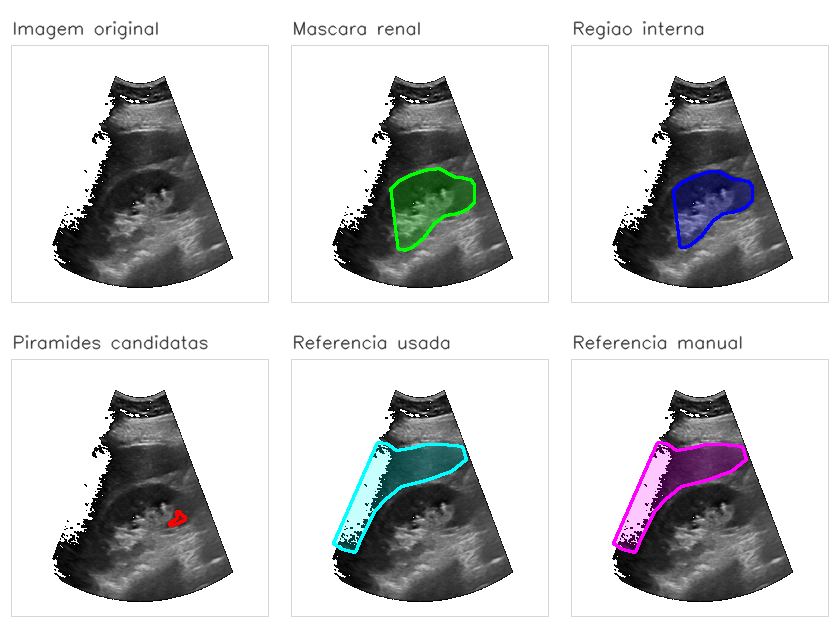
\includegraphics[width=0.5\textwidth]{figures/example_reference_high_ratio_1.png}
\caption{Exemplo de an\'alise com \'org\~ao de refer\^encia: imagem original, m\'ascara renal, regi\~ao intrarrenal, pir\^amides candidatas e ROIs de refer\^encia para compara\c{c}\~ao de ecogenicidade.}
\label{fig:reference_example}
\end{figure}

Na Figura~\ref{fig:reference_example}, a m\'ascara renal delimita a \'area em que os achados claros ser\~ao procurados. A regi\~ao intrarrenal e as pir\^amides candidatas organizam a busca espacial, enquanto as ROIs de refer\^encia permitem comparar a ecogenicidade do rim com o f\'igado quando essa informa\c{c}\~ao est\'a dispon\'ivel. Esse exemplo ilustra que a an\'alise n\~ao parte da imagem inteira, mas de uma regi\~ao anat\^omica segmentada.

\section{Resultados}

Para avaliar o efeito da expans\~ao do acervo no desempenho do segmentador, a Tabela~\ref{tab:segmentation_main} compara os resultados obtidos antes e depois da pseudorrotula\c{c}\~ao. Na etapa anterior, a escolha do DeepLabV3 R50 no \texttt{dataset\_augmented} foi orientada pela maior precis\~ao entre os modelos avaliados, com valor de \textbf{0,8426}.

\begin{table}[H]
\centering
\caption{Resultados de segmenta\c{c}\~ao antes e depois da expans\~ao do acervo.}
\label{tab:segmentation_main}
\resizebox{\textwidth}{!}{%
\begin{tabular}{lllccccc}
\hline
\textbf{Etapa} & \textbf{Modelo} & \textbf{Dataset} & \textbf{Dice} & \textbf{IoU} & \textbf{Prec.} & \textbf{Recall} & \textbf{FPS} \\
\hline
\multirow{4}{*}{Antes} & DeepLabV3 R50 & \multirow{4}{*}{\texttt{dataset\_augmented}} & 0,8472 & 0,7732 & \textbf{0,8426} & 0,8718 & 28,98 \\
 & SegFormer B2 &  & 0,8372 & 0,7700 & 0,8294 & 0,8782 & 35,66 \\
 & \mbox{U-Net} &  & 0,8119 & 0,7309 & 0,8039 & 0,8545 & 26,43 \\
 & UNet++ &  & 0,7924 & 0,6958 & 0,8189 & 0,7968 & 20,88 \\
\hline
Depois & DeepLabV3 R50 & \texttt{dataset\_geral} & \textbf{0,9235} & \textbf{0,8741} & \textbf{0,9301} & \textbf{0,9248} & 27,61 \\
\hline
\end{tabular}
}
\end{table}

Como mostra a Tabela~\ref{tab:segmentation_main}, depois da gera\c{c}\~ao de pseudom\'ascaras, da filtragem por confian\c{c}a de 90\% e do treinamento no \texttt{dataset\_geral}, o DeepLabV3 ResNet50 atingiu Dice m\'edio de 0,9235, IoU de 0.8741, precis\~ao de 0,9301 e recall de 0,9248 no teste fixo.

No \textit{pipeline} completo, essa melhora reduz a inclus\~ao de fundo, legenda e tecidos adjacentes, aumentando a confiabilidade das medidas intrarrenais. Esse ganho \'e relevante porque a busca por estruturas hiperecog\^enicas depende diretamente da qualidade da m\'ascara renal.

Para complementar a avalia\c{c}\~ao quantitativa, a Figura~\ref{fig:quality_good} mostra um exemplo qualitativo em um caso com contorno renal mais definido.

\begin{figure}[htb!]
\centering
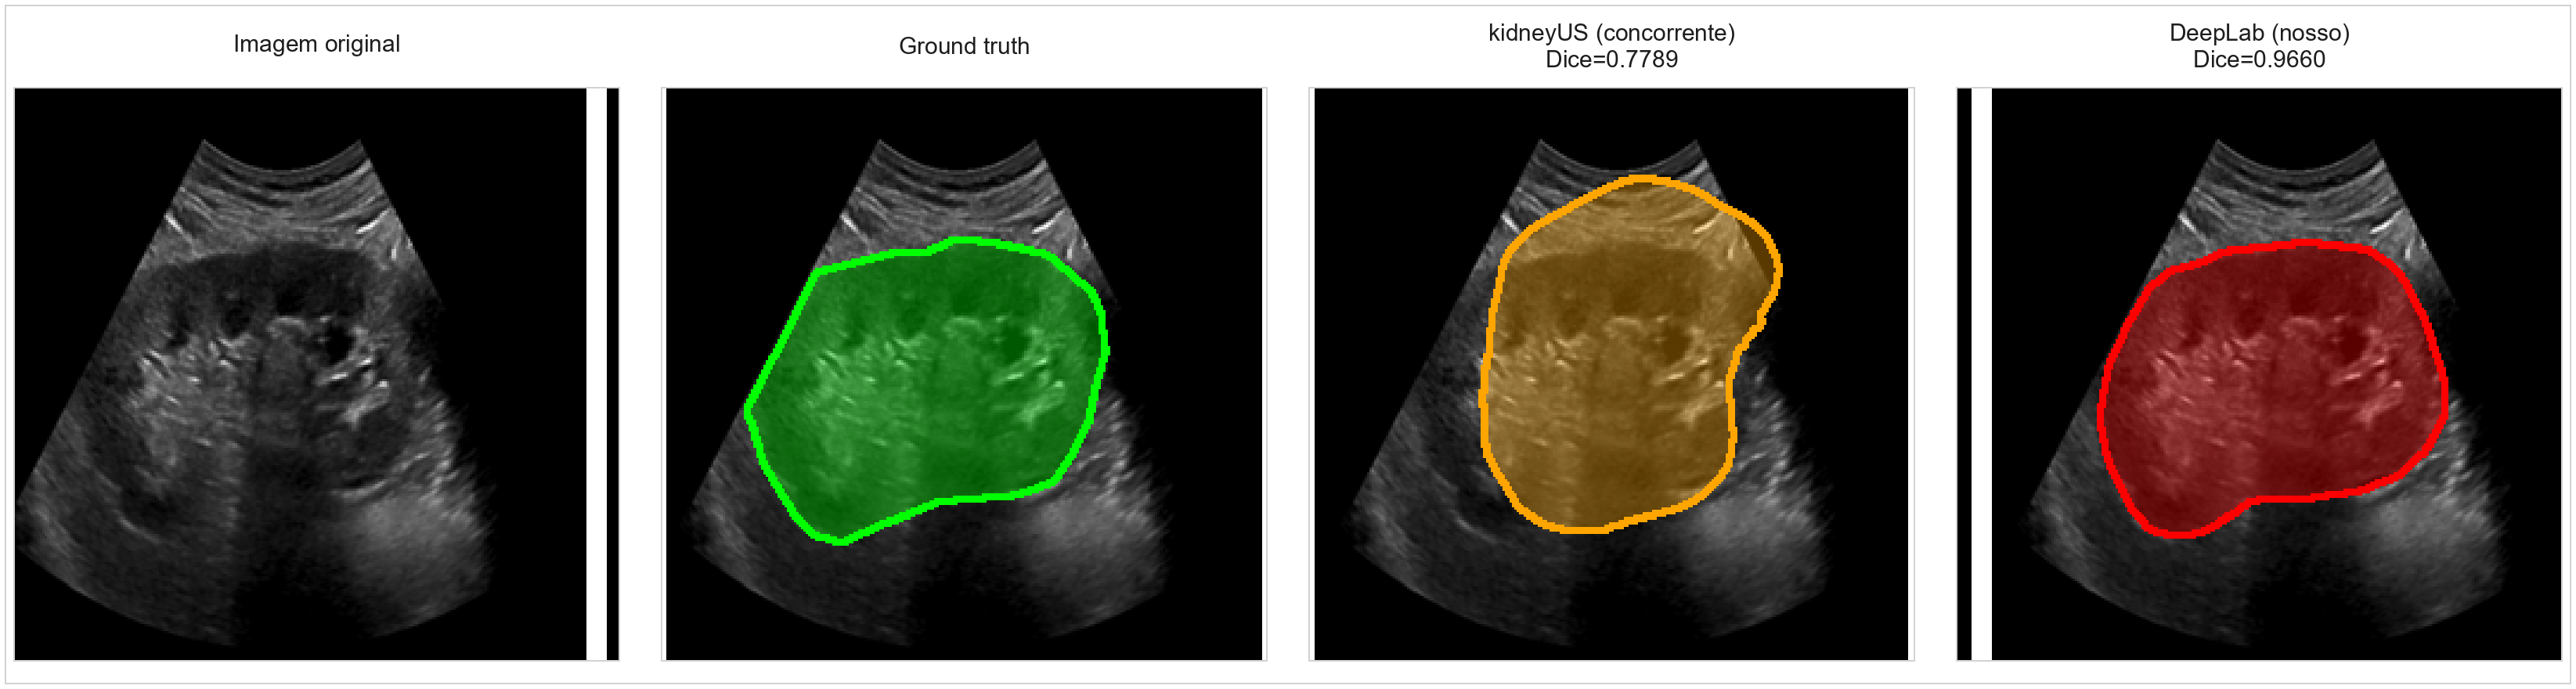
\includegraphics[width=0.45\textwidth]{figures/quality_good_comparison.png}
\caption{Caso qualitativo favor\'avel: imagem original, m\'ascara de refer\^encia, predi\c{c}\~ao do \texttt{kidneyUS} e predi\c{c}\~ao do DeepLab local.}
\label{fig:quality_good}
\end{figure}

Na Figura~\ref{fig:quality_good}, as colunas mostram a imagem original, a m\'ascara de refer\^encia, a predi\c{c}\~ao do modelo \texttt{kidneyUS} e a predi\c{c}\~ao do DeepLab treinado localmente. Com contorno renal mais definido, o modelo local recupera a geometria do rim com alta ader\^encia \`a refer\^encia. Essa estabilidade \'e importante porque a etapa seguinte depende de examinar apenas a regi\~ao renal, evitando que pontos brilhantes fora do rim sejam tratados como suspeitos.

Para ilustrar o uso do modelo de segmenta\c{c}\~ao 2 como entrada da prova de conceito, a Figura~\ref{fig:model2_proof} apresenta um caso em que a m\'ascara renal delimita a regi\~ao interna examinada e organiza as pir\^amides candidatas.

\begin{figure}[H]
\centering
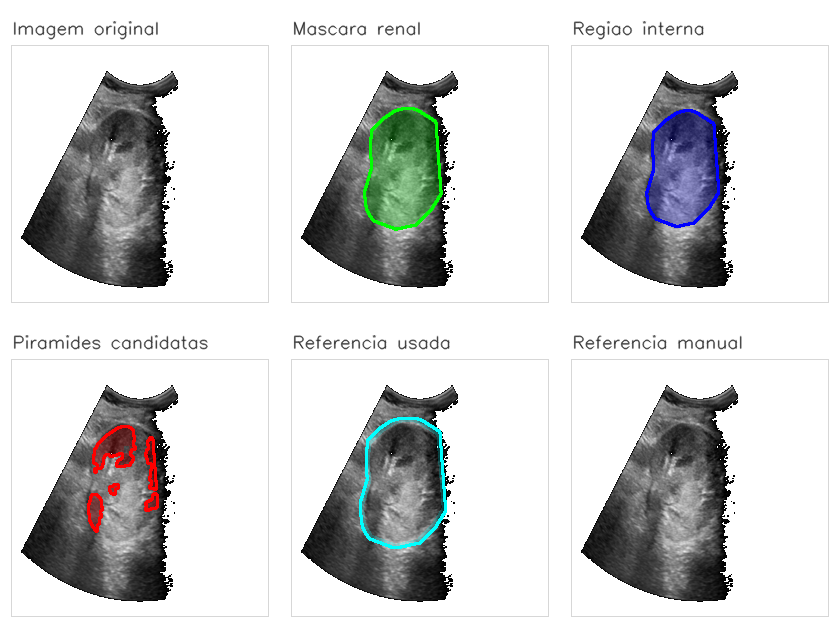
\includegraphics[width=0.40\textwidth]{figures/example_predicted_diseased_1.png}
\caption{Prova de conceito com o modelo de segmenta\c{c}\~ao 2: imagem original, m\'ascara renal, regi\~ao interna, pir\^amides candidatas e refer\^encias usadas na an\'alise.}
\label{fig:model2_proof}
\end{figure}

Na Figura~\ref{fig:model2_proof}, a sa\'ida do segundo segmentador n\~ao \'e tratada como diagn\'ostico final. Ela define a janela anat\^omica para extrair atributos de intensidade, textura e rela\c{c}\~ao espacial. Assim, a etapa posterior permanece uma caracteriza\c{c}\~ao explorat\'oria de marcadores ultrassonogr\'aficos; avaliar IFTA exigiria imagens associadas a bi\'opsia ou padr\~ao cl\'inico definido.

\section{Discussão}

Os resultados indicam que a principal contribuição do pipeline está na integração
entre segmentação anatômica e extração de atributos intrarrenais. A máscara renal
restringe a análise computacional ao órgão, reduzindo interferências externas e falsos
achados fora da anatomia renal.

A melhora observada após a expansão do acervo sugere que a pseudorrotulação pode ser útil em cenários médicos com poucas anotações especializadas. Embora o limiar de 90\% não substitua a validação clínica, ele funcionou como um mecanismo automático de controle de qualidade para a seleção das máscaras mais consistentes.

O pipeline também preserva a separação entre evidência computacional e interpretação clínica. Regiões hiperecogênicas não são tratadas como diagnóstico automático de fibrose, mas como achados candidatos para investigação quantitativa e validação posterior.

A comparação com resultados externos, como reproduções associadas ao
kidneyUS, deve ser feita com cautela devido a diferenças de resolução, anotação e distribuição dos exames. Ainda assim, os resultados preliminares indicam que o ajuste aos dados locais foi importante para aumentar a estabilidade das máscaras renais.

As principais limitações envolvem a ausência de um conjunto clínico robusto de fibrose, o pequeno número de exemplos rotulados e a falta de anotações manuais das pirâmides renais. Apesar disso, os resultados obtidos mostram que o pipeline já fornece uma base consistente para futuras investigações em análise ultrassonográfica renal.

\section{Conclus\~ao}

Este artigo prop\^os um \textit{pipeline} para isolar o rim e extrair marcadores ultrassonogr\'aficos intrarrenais explorat\'orios. A segmenta\c{c}\~ao foi constru\'ida em duas fases: modelo explorat\'orio inicial, gera\c{c}\~ao de pseudom\'ascaras com 90\% de confian\c{c}a e treinamento de um segundo modelo no \texttt{dataset\_geral}. Esse modelo alcan\c{c}ou Dice m\'edio de 0,9235 e sustenta a an\'alise intrarrenal.

Os resultados mostram que a segmentação pode restringir a análise computacional à anatomia renal, reduzindo interferências externas e aumentando a confiabilidade das medidas extraídas. A expansão supervisionada por pseudomáscaras também demonstrou potencial para ampliar o acervo de treinamento mesmo em cenários com limitação de
anotações manuais.

Al\'em do desempenho quantitativo, o \textit{pipeline} preserva a separa\c{c}\~ao entre evid\^encia computacional e interpreta\c{c}\~ao cl\'inica. Nesse contexto, as regi\~oes hiperecog\^enicas s\~ao tratadas como achados candidatos para investiga\c{c}\~ao, e n\~ao como diagn\'ostico autom\'atico. Uma etapa de predi\c{c}\~ao de IFTA depende de casos vinculados a padr\~ao histol\'ogico ou cl\'inico validado.

Como trabalhos futuros, pretende-se ampliar o conjunto anotado, incluir marcações específicas das pirâmides renais e validar os atributos extraídos em cenários clínicos reais. Também se pretende investigar estratégias semi-supervisionadas e avaliar a integração de informações clínicas e medidas relativas de ecogenicidade para aumentar a robustez da análise.


\newpage
\bibliographystyle{sbc}
\bibliography{sbc-template}

\end{document}
